\documentclass[conference]{IEEEtran}
\IEEEoverridecommandlockouts
% The preceding line is only needed to identify funding in the first footnote. If that is unneeded, please comment it out.
\usepackage{cite}
\usepackage{amsmath,amssymb,amsfonts}
\usepackage{algorithmic}
\usepackage{graphicx}
\usepackage{textcomp}
\usepackage{xcolor}
\usepackage{float}
\graphicspath{ {./packet_structure.png/} {./receive_packet.png/} }
\def\BibTeX{{\rm B\kern-.05em{\sc i\kern-.025em b}\kern-.08em
    T\kern-.1667em\lower.7ex\hbox{E}\kern-.125emX}}
\begin{document}

\title{CENG 435 Term Project Part 2 - Group 83 Report\\
{\footnotesize \textsuperscript{*}}
\thanks{}
}
\author{\IEEEauthorblockN{ KAAN KALAYCIOGLU}
\IEEEauthorblockA{\textit{Computer Engineering Department} \\
{Middle East Technical University}\\
Ankara,Turkey \\
e2237519@ceng.metu.edu.tr}
\and
\IEEEauthorblockN{YUSIF ALIYEV}
\IEEEauthorblockA{\textit{Computer Engineering Department} \\
{Middle East Technical University}\\
Ankara,Turkey \\
e1949940@ceng.metu.edu.tr}
}

\maketitle

\begin{abstract}
In the first part of Term Project we constructed User Datagram Protocol(UDP) in the Topology that we created on the GENI Platform. However, in the second part, that is-in this part we designed and implemented our own Reliable Data Transfer Protocol(RDT) using UDP in order to make the UDP reliable. We created our own UDP-based RDT protocol which is different from the RDT 3.0 and etc. and that supports Pipelining and Multi-homing.  
\end{abstract}

\begin{IEEEkeywords}
User Datagram Protocol(UDP), Reliable Data Transfer (RDT),File Transfer Time(FTT), Pipelining,Multi-homing, UDP Sockets, Socket Programming,Data Packets, Header,  Checksum, Sequence Number, ACK mechanism, Packet Loss.
\end{IEEEkeywords}

\section{Introduction}
In this project, we are expected to design and implement our own Reliable Data Transfer Protocol(RDT) based on the User Datagram Protocol(UDP) over a network consisting of 5 nodes that using this protocol we are expected to transfer a large file from Source node to Destination node using the shortest path between the Source node and the Destination node which was Source- R3-Destination that we obtained from the first part of the Term Project. Then, we are expected to do experiments over this network and protocol, such as we should stimulate the package loss by given commands with 3ms delay and File Transfer Time (FTT) with $95\%$ confidence intervals and margin error should be less than $2.5\%$ with the z-score equal to $1.96$ and we should find the value of $n$ which is the number of repetition of each experiment explicitly. In addition to this, we are expected to represent the result of the experiments as a bar graph or a line chart.

\section{Design Approach}



We have agreed on to write our scripts in Python because it is simple and easy to integrate for different inputs , arguments and etc and has lots of useful libraries. We have decided to write scripts for the shortest path we found at the first part of Term Project : Source Node - R3 Node - Destination Node explicitly and named them as $Sender.py$ for Source Node , $Forward.py$  for R3 Node and  $Receiver.py$ for the Destination Node. 
\subsection{Sender Script}\label{AA}

In Sender(at the Source Node) UDP connection established with the help of Socket programming and the large input file is parsed into segments(we named them as $data$) such that each segment size chosen as 996 bytes in order not to exceed the max packet size limit (in our project it is determined as 1000 bytes), because after parsing the file and storing them in the array in order to reach them as indexed parts in future, we are adding the header bytes consisting of $checksum$,  $sequence$ $number$. For computing the checksum we decided to import the $Md5$ library of Python because there is a method named as $hashlib$ that takes the data which you want to add them in the computation of checksum, and the function returns the checksum value. Later we take it and append it to the packet at Sender. We used the built in $time()$ function of the Python to keep track of the time in order to compute the FTT and the time-outs of the sockets and last "ACKed" packet and etc. that will be explained in detail in Implementation part. We designed $pipelining$ as windows size chosen as 20, base index starting from 0 and incremented according to the last "ACKed" packet and a $window$ $array$ that we store the packets in it. Then, put the necessary packets according to our implementation, into the $sendSocket$ that sends packets to the $Forward$ script in the R3 node. At the same time, $Sender$ script also have the $recvSocket$ that receives packet consisting of expected sequence number and checksum from the $Forward$ script in order to maintain the order of packets. Then , we designed the script in a way that takes this expected sequence number and re-sends the expected packets and after "understanding" that packed ACKed, window's base index incremented accordingly. Finally, if the end of the file is reached, we append "END" string to the last packet and send it to the Forward Node.  
\subsection{Forward Script}\label{BB}
As mentioned above, in R3 node, Forward script is running. Basically, we designed the Forward script to do 4 tasks with UDP implementation. We used Socket Programming and Threading to listen and receive packets from the nodes Source and Destination at the same time. This script's main purpose is forwarding the coming packets to appropriate locations. The reason why we design to use Threading is that , R3 Node should be listening to the Source Node at the same time it should send the packets coming from the Source Node (forwarding) to the Destination Node, also, it should be listening to the Destination Node and forwarding the coming packets from this node to the Source Node and all of this processes should be executed simultaneously and synchronically. Moreover, we design four sockets in the two functions named $receiveSforwardD$ and $receieveDforwardS$ and in the first one it contains two sockets that one of it listening to the Source node and the other is sending the coming packet from it to the Destination node. Second one also contains two sockets that one of it listening to the Destination node and the other is sending the coming packets from it to the Source node.

\subsection{Receiver Script}\label{CC}
$Receiver.py$ Script is running on the Destination Node. We also designed UDP connection with the help of Socket Programming like in the Sender node. Two sockets are designed. First one is $recvSock$ is that it is receiving(listening to) the coming packets from R3 Node and the other one is $send_Sock$ is that it sends the last in order received packet's sequence number as an ACK message or the last Not In Ordered packet's expected sequence number to the Forward(R3) Node. For the coming packets, we designed our script in a way that first it should check the coming packet's checksum value. We are using the Python's $Md5$ library's $hashlib()$ function to check the checksum value. If it is not corrupted, then we check the sequence number of the coming packet with the expected sequence number which is initially started from value 1 and then if they are equal to each other then, it means the packet is received In Order and "received in order" message with the sequence number is printed on the terminal and the packet is parsed , the actual data will be taken and written on the output file. If not, the packet received Not In Order , "received not in order" message with the sequence number displayed in terminal. Then the new packet is created with the expected sequence number and with the checksum then it will be transferred to the $send_Sock$ to the Forward Node. Additionally with the help of Pythons $time()$ function , we keep track of time in order to compute the FTT and time-outs for the packets if the expected packet does not arrive. If packet does not arrive after time-out ends, expected sequence number and the checksum value computed and appended to new packet and sent to the $send_Socket$ to the Forward Node. Finally, we check the end of transfer of the large file by looking for the "END" string in the coming packets, if yes,"File Transfer Successful" message will be displayed. After that, end time will be taken and FTT will be measured.

\section{Implementation}
\subsection{Sender Node}
Since we were asked to implement our own reliable data protocol over UDP firstly, we open a UDP socket between the Source Node and the Forward(R3 Node) in order to send packets and listen for ACKs. Sender script takes IP address and port numbers at command line as arguments as well as the large file to be sent. These arguments discussed in more detail in the $Readme.txt$ file.  In the packet we send to the destination, we have the sequence number, payload(data) and the checksum calculated using the payload and sequence number data. We calculate the checksum using the  $hashlib()$ function from $Md5$ library of Python module.That is, first we take the data that is parsed from the input file and the sequence number we will assign to the packet, send it to the $hashlib()$ function, then store it to a variable to append the calculated checksum to the header of the packet. We transform this packet into a compact byte stream using the $pickle$ module. Code for this process can be seen below.

\begin{figure}[H]
  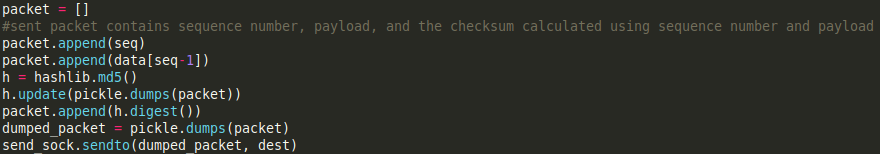
\includegraphics[width=\linewidth]{packet_structure.png}
  \caption{Code for creating the packet structure.}
  \label{fig:packet}
\end{figure}

After creating the packet we send it to the destination over Forward node without waiting for the ACK response.The code waits for the sequence number of the ACKed packet. Then, when the sequence number returns, we slide the window up to that sequence number index at the window. If the ACK response is not received within a given period of time(defined it as time-out ends after 0.2 seconds), we send every packet in the window again. This process goes on until the last packet sent is ACKed by the receiver node. $Done$ flag implemented in order to know the end of file and it is initiated as $false$. If the last data segment reached, done flag setting as $true$ we create the last packet consisting of that data, sequence number, checksum and finally we append the "END" string to that packet and send it to indicate the end of file. Also we keep track of the time  with the help of the built-in $time$ function of Python in order to compute the FTT. For that purpose, just before the first packet sends we takes the time and store it in the $startTime$ variable. Also, we are using the time() function to store the last ACKed packet's time to compute the time-out for the not received ACKs and send every packet in the window. 
\subsection{Receiver Node}
In the receiver node the UDP socket approach is the same with the sender node. We read the corresponding IP addresses and ports as a command line argument. After the sockets are set correctly receiver node starts waiting for packets to arrive from the Sender node. When a packet arrives this node , firstly it verifies the checksum. If the checksum is correct (by using hashlib() function)the node proceeds to checking of sequence number. If the sequence number is not equal to the expected sequence number the packet is dropped and a new packet created with the expected sequence number and with the new calculated checksum is sent to the sender node. If the sequence number is the expected sequence number the packet is extracted and payload(data) is written to the output file. Code for the verification process can be seen below.

\begin{figure}[H]
  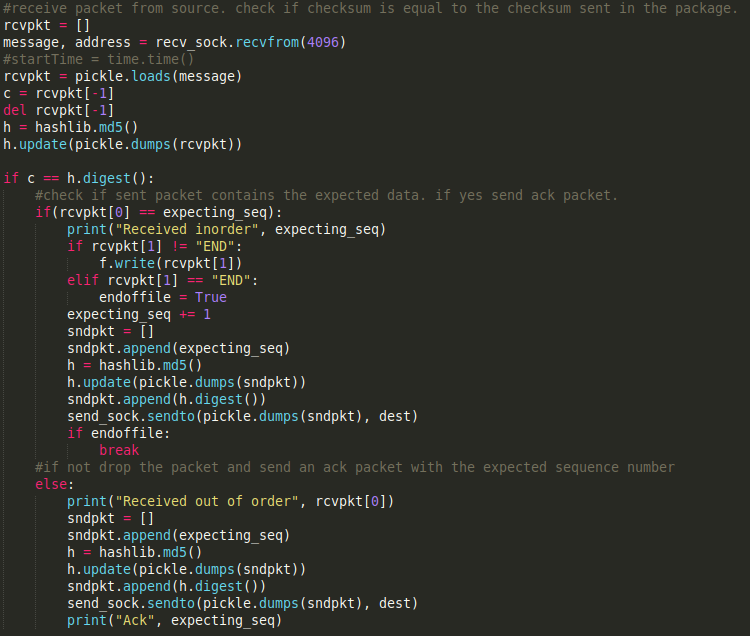
\includegraphics[width=\linewidth]{receive_packet.png}
  \caption{Code for checking the sequence number and checksum in the receiver node.}
  \label{fig:receive}
\end{figure}
Then,  if $endoffile$ flag sets as $true$ when the received packet contains "END" string ,that means the end of file is reached. At the end of the file transfer the Receiver node computes the time taken to transfer the file and writes the result into a file named "times.txt". This file is used in the calculations of the confidence interval of different packet loss percentages. Script terminates after the write operation is completed.

\subsection{Forward Node}
This node acts as a forwarder that receives packet from the sender node and transfer it to the receiver node. This script runs in the R3 Node. As command line gives  argument, this script takes IP addresses and Port numbers of the corresponding interfaces between s-r3 and r3-d. There is a Thread structure in this script for handling the connection between s-r3 and r3-d. Thread for s-r3 link listens for a packet from the Sender Node. When the packet is received it is forwarded to the Receiver node by $receiveSforwardD$ function that contains the appropriate sockets explained in Design part. This is also the case for the r3-d Thread, such as the packets received from Destination node and forwarded to the Source Node by $receiveDforwardS$ function that runs in r3-d Thread. We used the built-in threading module in python to accomplish the threaded structure with $thread.start()$ and $thread.join()$ functions. 

\section{Experiment}
For the first experiment we set the delay as 3ms and the packet loss percentage as 5 percent using the following [sudo tc qdisc add dev eth0 root netem ]and [sudo tc qdisc change dev eth0 root netem loss 5\% delay 3ms] commands. This command is used for all nodes in the topology and every interface of each node. We run our script 20 times to calculate the confidence interval,so $n=20$. Mean of our 20 samples is 244.7 seconds and the standard deviation is 4.28 . We used a tool called Confidence Interval Calculator to calculate our confidence interval. Our confidence is [244.7-1.877, 244.7+1.877]. As specified in the assignment our error margin is less than \%2.5 which is \%1.877 . After adding the loss percentage and delay to our nodes we observed that file transfer time has increased a lot. So we conclude that loss percentage is directly proportional to the file transfer time.

We increased the packet loss percentage to \%15 and run our scripts again. However, the file transfer time increased greatly. Because of this we weren't able to obtain enough samples to calculate a confidence interval for other packet loss configurations.


\section{Conclusion}
In this part of the Term Project , we managed to create a Reliable Data Transfer Protocol(RDT) on top of the User Datagram Protocol(UDP) using Pipelining with implementing Go-Back-N with the window size equal to 20. In order to make our protocol reliable, we used the checksum value, expected sequence numbers of the packets (for ACK), to control the data dransfer we used flags to indicate end of file, used time() function to keep track of the FTT and  last ACKed packet's time to compute the time-out for the not received ACKs and re-sending from the last ACKed packet's index in the window array. For the experiment part, we experimented 5\% packet loss and measure the sample size n=20 and calculated the Confidence Interval and achieve the error margin less than 2.5 \% . Hovewer, unfortunately, when increasig the packet loss percentage, our experiment slows down significantly that we are unable to measure the sample size for the higher packet loss percentages because it took so much time to compute. Therefore, we stick to the 5\% packet loss and achieved the error margin less than 2.5\% (found 1.877 \%) also for this reason we could not plot graphs. However , at the end of day we can say that we achieved to manage Reliable Data Transfer between the Source,R3 and Destination Nodes using UDP and experimented 5\% packet loss successfully. 

\section{References}
1) https://www.mathsisfun.com/data/confidence-interval-calculator.html


\end{document}

